
\chapter{The Top Physics and Machine Learning}

\section{The Top Physics}

Top quark, the most massive fundamental particle in Standard Model(SM), is the only quark that decays semi-weakly (i.e.~decay into a W bonson and bottom quark). Its large mass leads to a short lifetime and decay before hadronization occurs. Top quark contains many interesting properties, such as its mass, couplings, and cross-section, etc. The accurate measurement these properties will facilitate understanding of fundamental interactions and provide the key to Beyond Standard Model\cite{Zyla:2020zbs}.
\\
In the Standard Model, a top quark pair produced by $pp$ collision has three decay modes, \textbf{all hadronic channel}, \textbf{semi-leptonic channel}, and \textbf{dileptonic channel}. The branching ratios of each channel are shown in Table \ref{table:Branchratio}. The decay width of a top-quark predicted in SM is\cite{A.Quadt:2008TopPhysics}: 
\begin{equation}
	\Gamma_{t} = \frac{G_{F}m_{t}^{3}}{8\pi\sqrt{2}}\left(1-\frac{M_{W}^{2}}{m_{t}^{2}}\right)^{2}\left(1+2\frac{M_{W}^{2}}{m_{t}^{2}}\right)\times\left[1 - \frac{2\alpha_{s}}{3\pi}\left( \frac{2\pi^{2}}{3} - \frac{5}{2}\right) \right].
\end{equation}
\\
\begin{center}
\begin{table}[h]
\begin{tabular}{ c c c}
	\cline{1-3}
	Decay Channel    & Process & Branch Ratio(\%) \\
	\hline
	All-hadronic      & $t\bar{t}\to W^{+}bW^{-}\bar{b}\to q\bar{q}'bq''\bar{q}'''\bar{b}$    & 45.7     \\
	Semi-leptonic       &   $t\bar{t}\to W^{+}bW^{-}\bar{b}\to q\bar{q}'b\ell^{-}\bar{\nu}_{\ell}\bar{b} + \ell^{+}\nu_{\ell}bq''\bar{q}'''\bar{b}$   & 43.8     \\
	Dileptonic      &   $t\bar{t}\to W^{+}bW^{-}\bar{b}\to \ell^{+}\nu_{\ell}b\ell'\bar{\nu}_{\ell'}\bar{b}$   & 10.5      \\
	\hline
\end{tabular}
\caption{Top quark pair decay processes\cite{Zyla:2020zbs}.}
\label{table:Branchratio}
\end{table}
\end{center}
In recent study, the most precise result of the top quark mass is measured in the lepton+jets channel due to its good signal-to-background ratio and the presence of one neutrino final state\cite{Mccarthy:2015ucy}. Although the all-hadronic channel has the most probability to appears in the top quark pair decay process, its poor signal-to-background ratio renders inaccurate mass measurements owing to the difficult QCD background. The CMS and ATLAS group approach a precision of the top mass measurement using the all-hadronic channel with uncertainties of 0.65\% and 1.1\%\cite{Sirunyan:2018mlv}\cite{Aaboud:2017mae}.
\\
\newline
In this project, we focus on the \textbf{jet-parton assignment problem in all hadronic decay channel}, becuase of the resolved 6 jets signature and the potential of the machine learning method to apply to the ambiguous event reconstruction problem. There exist six jets in the final state, two b-jets and four quark jets, they can be separated into two groups $\left(b, q, \bar{q}\right)$ and $\left(\bar{b}, q, \bar{q}\right)$. The schematic of the decay products is shown in Figure  \ref{fig:ttbardecaymode}. 
\begin{figure}[h]
	\centering
	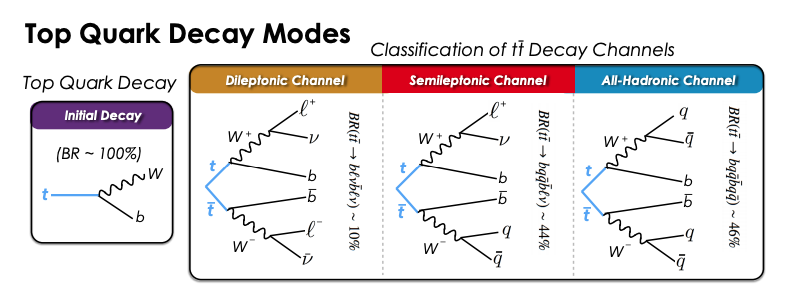
\includegraphics[width=0.8\linewidth]{Figures/ttbar-decay-mode.png}
	\caption{The schematic of Top quark decay channels\cite{Mccarthy:2015ucy}. Due to its characteristic, it will decay into W boson and b quark almost 100\%. Considering the decay channel of W boson, there are three combinations that forming the final states of fully hadronic top decay.}
	\label{fig:ttbardecaymode}
\end{figure}
\section{Machine Learning and its application on Particle Physics}
Machine Learning techniques have practical applications in many fields (e.g.~Computer Vision, Solving PDE, Medical analysis, etc.) in recent age, including particle physics. From the search of the higgs boson (neural network and BDT) to the b-tagging technology (BDT\cite{Paganini:2017dpd}), physicists have already applied several kinds of machine learning methods to recent research.
\\
In a nutshell, machine learning can break into several cases; it can help to do classification, regression, and clustering problems. ML cannot only accelerate the computation of well-defined problems, but also help to find new path to unsolved area. This project utilizes the state-of-the-art machine learning technology, the attention mechanism\cite{A.Vaswani:2017}, a technology based on the evolution of Recurrent Neural Networks (RNN)\cite{A.Vaswani:2017}. The attention mechanism not only consider the local relationship and the sequence neighbor but also calculates the global relation base on the self-attention calculation shown in Figure \ref{fig:attention}. Using this novel architecture, we will train on the relationship between each jet and try to figure out the correct information of the top quark pairs.
\\
\begin{figure}[h]
	\centering
	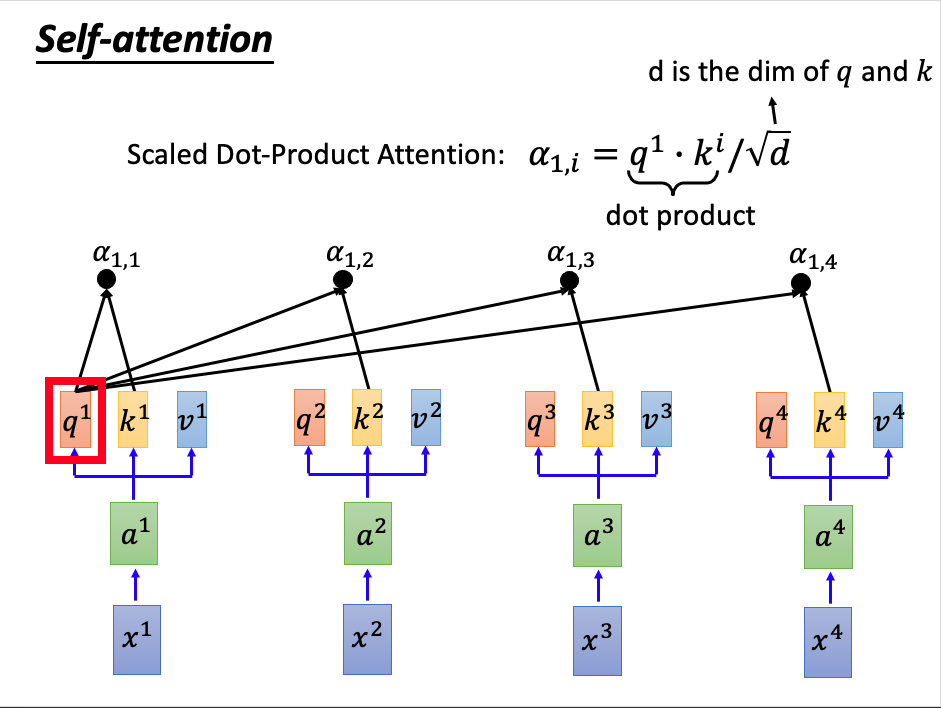
\includegraphics[width=0.7\linewidth]{Figures/attention.png}
	\caption{A demonstration of how self-attention works\cite{HY.Lee:2019}. The basic of attention is to decompose the input sequence into three bases. The network will extract the information from these bases. The computation shown in figure is a stage that computing the attention score between each elements in a sequence.}
	\label{fig:attention}
\end{figure}
